\documentclass{article}
\usepackage[utf8]{inputenc}
\usepackage[french]{babel}
\usepackage[margin=2cm]{geometry}
\usepackage{multicol}
\usepackage{graphicx}
\usepackage{float}
\usepackage{adjustbox}

\begin{document}
\section{Introduction}
\section{Présentation des données}
\singlespacing
\clearpage \subsection{pud} 
 \begin{itemize} 
 \item[Présentation :] Phrases qui proviennent de sites informatifs, id est de journaux ou de Wikipedia

 \item[Pourcentage de mots hors vocabulaire : ]54.04
 \item[KL-Divergence :]0.256
 \end{itemize}  \subparagraph{Données de test \\ }  
 Nombre de phrases : 1000\\ 
\begin{figure}[H] \begin{minipage}{0.48\textwidth} \centering \begin{tabular}{|l || *{11 }{|c} |} \hline
Mot & Apparitions  \\ \hline
\begin{verb} , \end{verb} &1178\\ \hline
\begin{verb} de \end{verb} &1175\\ \hline
\begin{verb} . \end{verb} &985\\ \hline
\begin{verb} la \end{verb} &675\\ \hline
\begin{verb} et \end{verb} &442\\ \hline
\begin{verb} le \end{verb} &414\\ \hline
\begin{verb} les \end{verb} &399\\ \hline
\begin{verb} à \end{verb} &370\\ \hline
\begin{verb} l' \end{verb} &328\\ \hline
\begin{verb} des \end{verb} &327\\ \hline

\end{tabular}
\caption{ Mots les plus utilisés dans le set pud(test) } \label{Fig:muw}\end{minipage} 
\begin{minipage}{0.48\textwidth} \centering
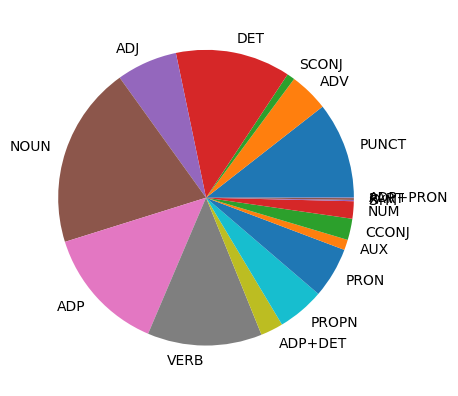
\includegraphics[width=.7\linewidth]{pudtest_img.png}
\caption{distribution des labels}
\end{minipage}
\end{figure} \subparagraph{Données de train \\ }  
 Nombre de phrases : 803\\ 
\begin{figure}[H] \begin{minipage}{0.48\textwidth} \centering \begin{tabular}{|l || *{11 }{|c} |} \hline
Mot & Apparitions  \\ \hline
\begin{verb} de \end{verb} &1114\\ \hline
\begin{verb} , \end{verb} &1016\\ \hline
\begin{verb} . \end{verb} &750\\ \hline
\begin{verb} la \end{verb} &683\\ \hline
\begin{verb} et \end{verb} &544\\ \hline
\begin{verb} l' \end{verb} &486\\ \hline
\begin{verb} des \end{verb} &432\\ \hline
\begin{verb} à \end{verb} &404\\ \hline
\begin{verb} d' \end{verb} &397\\ \hline
\begin{verb} le \end{verb} &385\\ \hline

\end{tabular}
\caption{ Mots les plus utilisés dans le set pud(train) } \label{Fig:muw}\end{minipage} 
\begin{minipage}{0.48\textwidth} \centering
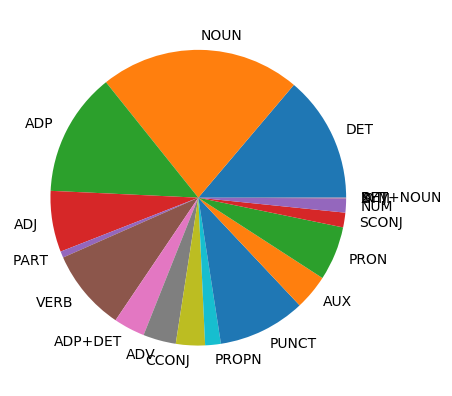
\includegraphics[width=.7\linewidth]{pudtrain_img.png}
\caption{distribution des labels}
\end{minipage}
\end{figure}


\clearpage \subsection{ftb } 
 \begin{itemize} 
 \item[Présentation :] Phrases provenant du journal «Le Monde»

 \item[Pourcentage de mots hors vocabulaire : ]7.099
 \item[KL-Divergence :]0.110
 \end{itemize}  \subparagraph{Données de test \\ }  
 Nombre de phrases : 2541\\ 
\begin{figure}[H] \begin{minipage}{0.48\textwidth} \centering \begin{tabular}{|l || *{11 }{|c} |} \hline
Mot & Apparitions  \\ \hline
\begin{verb} , \end{verb} &4528\\ \hline
\begin{verb} de \end{verb} &3593\\ \hline
\begin{verb} . \end{verb} &2258\\ \hline
\begin{verb} __DIGIT__ \end{verb} &2200\\ \hline
\begin{verb} la \end{verb} &2016\\ \hline
\begin{verb} l' \end{verb} &1350\\ \hline
\begin{verb} à \end{verb} &1333\\ \hline
\begin{verb} le \end{verb} &1293\\ \hline
\begin{verb} des \end{verb} &1255\\ \hline
\begin{verb} les \end{verb} &1222\\ \hline

\end{tabular}
\caption{ Mots les plus utilisés dans le set ftb(test) } \label{Fig:muw}\end{minipage} 
\begin{minipage}{0.48\textwidth} \centering
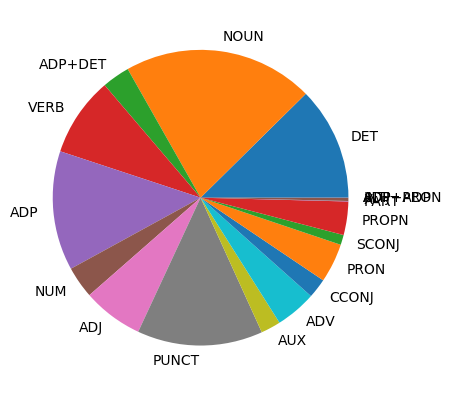
\includegraphics[width=.7\linewidth]{ftbtest_img.png}
\caption{distribution des labels}
\end{minipage}
\end{figure} \subparagraph{Données de train \\ }  
 Nombre de phrases : 14759\\ 
\begin{figure}[H] \begin{minipage}{0.48\textwidth} \centering \begin{tabular}{|l || *{11 }{|c} |} \hline
Mot & Apparitions  \\ \hline
\begin{verb} , \end{verb} &27318\\ \hline
\begin{verb} de \end{verb} &22518\\ \hline
\begin{verb} . \end{verb} &13735\\ \hline
\begin{verb} __DIGIT__ \end{verb} &11104\\ \hline
\begin{verb} la \end{verb} &10780\\ \hline
\begin{verb} l' \end{verb} &8129\\ \hline
\begin{verb} à \end{verb} &7984\\ \hline
\begin{verb} le \end{verb} &7255\\ \hline
\begin{verb} les \end{verb} &7086\\ \hline
\begin{verb} des \end{verb} &7071\\ \hline

\end{tabular}
\caption{ Mots les plus utilisés dans le set ftb(train) } \label{Fig:muw}\end{minipage} 
\begin{minipage}{0.48\textwidth} \centering
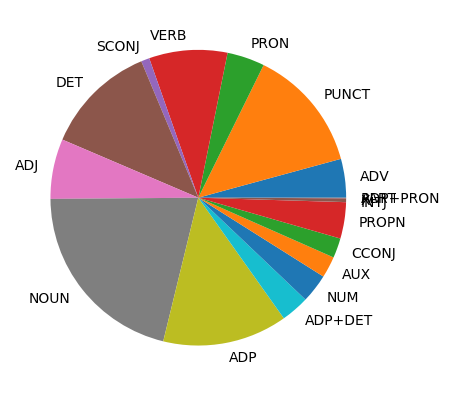
\includegraphics[width=.7\linewidth]{ftbtrain_img.png}
\caption{distribution des labels}
\end{minipage}
\end{figure}


\clearpage \subsection{spoken } 
 \begin{itemize} 
 \item[Présentation :] Données sur le français oral

 \item[Pourcentage de mots hors vocabulaire : ]32.14
 \item[KL-Divergence :]0.366
 \end{itemize}  \subparagraph{Données de test \\ }  
 Nombre de phrases : 726\\ 
\begin{figure}[H] \begin{minipage}{0.48\textwidth} \centering \begin{tabular}{|l || *{11 }{|c} |} \hline
Mot & Apparitions  \\ \hline
\begin{verb} de \end{verb} &380\\ \hline
\begin{verb} est \end{verb} &262\\ \hline
\begin{verb} euh \end{verb} &222\\ \hline
\begin{verb} la \end{verb} &219\\ \hline
\begin{verb} et \end{verb} &193\\ \hline
\begin{verb} que \end{verb} &188\\ \hline
\begin{verb} le \end{verb} &181\\ \hline
\begin{verb} l' \end{verb} &177\\ \hline
\begin{verb} à \end{verb} &169\\ \hline
\begin{verb} je \end{verb} &162\\ \hline

\end{tabular}
\caption{ Mots les plus utilisés dans le set spoken(test) } \label{Fig:muw}\end{minipage} 
\begin{minipage}{0.48\textwidth} \centering
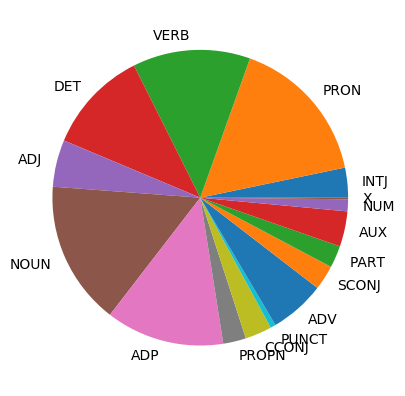
\includegraphics[width=.7\linewidth]{spokentest_img.png}
\caption{distribution des labels}
\end{minipage}
\end{figure} \subparagraph{Données de train \\ }  
 Nombre de phrases : 1153\\ 
\begin{figure}[H] \begin{minipage}{0.48\textwidth} \centering \begin{tabular}{|l || *{11 }{|c} |} \hline
Mot & Apparitions  \\ \hline
\begin{verb} de \end{verb} &529\\ \hline
\begin{verb} euh \end{verb} &489\\ \hline
\begin{verb} est \end{verb} &362\\ \hline
\begin{verb} la \end{verb} &339\\ \hline
\begin{verb} et \end{verb} &328\\ \hline
\begin{verb} le \end{verb} &294\\ \hline
\begin{verb} à \end{verb} &282\\ \hline
\begin{verb} c' \end{verb} &264\\ \hline
\begin{verb} je \end{verb} &223\\ \hline
\begin{verb} qui \end{verb} &218\\ \hline

\end{tabular}
\caption{ Mots les plus utilisés dans le set spoken(train) } \label{Fig:muw}\end{minipage} 
\begin{minipage}{0.48\textwidth} \centering
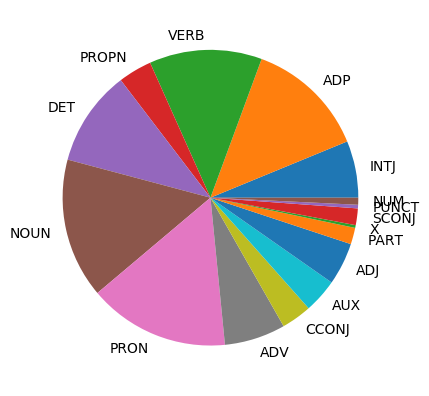
\includegraphics[width=.7\linewidth]{spokentrain_img.png}
\caption{distribution des labels}
\end{minipage}
\end{figure}


\clearpage \subsection{sequoia } 
 \begin{itemize} 
 \item[Présentation :] Ensemble de texte, à la base disponible avec des annotations «profondes», ie plus complètes. Néanmoins, ces annotations ont été normalisées par rapport aux autres données

 \item[Pourcentage de mots hors vocabulaire : ]9.417
 \item[KL-Divergence :]0.113
 \end{itemize}  \subparagraph{Données de test \\ }  
 Nombre de phrases : 456\\ 
\begin{figure}[H] \begin{minipage}{0.48\textwidth} \centering \begin{tabular}{|l || *{11 }{|c} |} \hline
Mot & Apparitions  \\ \hline
\begin{verb} de \end{verb} &463\\ \hline
\begin{verb} , \end{verb} &431\\ \hline
\begin{verb} . \end{verb} &344\\ \hline
\begin{verb} la \end{verb} &216\\ \hline
\begin{verb} __DIGIT__ \end{verb} &204\\ \hline
\begin{verb} l' \end{verb} &186\\ \hline
\begin{verb} à \end{verb} &169\\ \hline
\begin{verb} et \end{verb} &165\\ \hline
\begin{verb} des \end{verb} &152\\ \hline
\begin{verb} d' \end{verb} &139\\ \hline

\end{tabular}
\caption{ Mots les plus utilisés dans le set sequoia(test) } \label{Fig:muw}\end{minipage} 
\begin{minipage}{0.48\textwidth} \centering
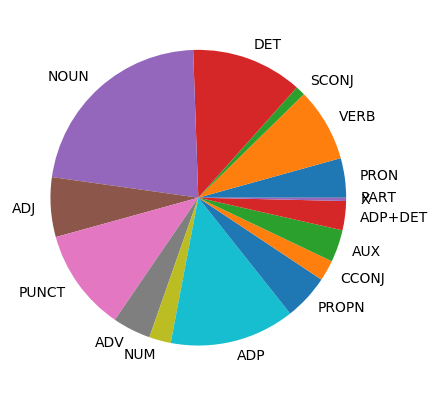
\includegraphics[width=.7\linewidth]{sequoiatest_img.png}
\caption{distribution des labels}
\end{minipage}
\end{figure} \subparagraph{Données de train \\ }  
 Nombre de phrases : 2231\\ 
\begin{figure}[H] \begin{minipage}{0.48\textwidth} \centering \begin{tabular}{|l || *{11 }{|c} |} \hline
Mot & Apparitions  \\ \hline
\begin{verb} de \end{verb} &2435\\ \hline
\begin{verb} , \end{verb} &2354\\ \hline
\begin{verb} . \end{verb} &1683\\ \hline
\begin{verb} la \end{verb} &1176\\ \hline
\begin{verb} __DIGIT__ \end{verb} &1039\\ \hline
\begin{verb} l' \end{verb} &916\\ \hline
\begin{verb} à \end{verb} &857\\ \hline
\begin{verb} et \end{verb} &845\\ \hline
\begin{verb} des \end{verb} &759\\ \hline
\begin{verb} le \end{verb} &743\\ \hline

\end{tabular}
\caption{ Mots les plus utilisés dans le set sequoia(train) } \label{Fig:muw}\end{minipage} 
\begin{minipage}{0.48\textwidth} \centering
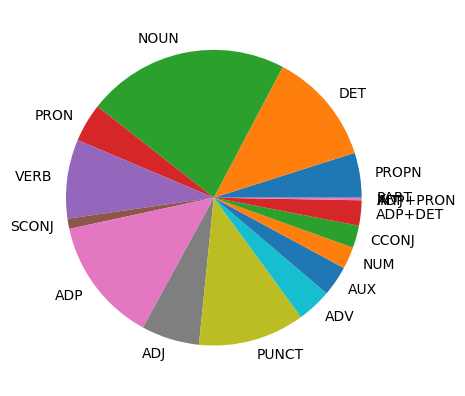
\includegraphics[width=.7\linewidth]{sequoiatrain_img.png}
\caption{distribution des labels}
\end{minipage}
\end{figure}


\clearpage \subsection{partut } 
 \begin{itemize} 
 \item[Présentation :] Ensemble varié de textes, incluant de extraits de conférences comme des extraits de Wikipedia ou des textes légaux

 \item[Pourcentage de mots hors vocabulaire : ]5.743
 \item[KL-Divergence :]0.330
 \end{itemize}  \subparagraph{Données de test \\ }  
 Nombre de phrases : 110\\ 
\begin{figure}[H] \begin{minipage}{0.48\textwidth} \centering \begin{tabular}{|l || *{11 }{|c} |} \hline
Mot & Apparitions  \\ \hline
\begin{verb} de \end{verb} &120\\ \hline
\begin{verb} . \end{verb} &110\\ \hline
\begin{verb} , \end{verb} &79\\ \hline
\begin{verb} la \end{verb} &69\\ \hline
\begin{verb} à \end{verb} &58\\ \hline
\begin{verb} l' \end{verb} &56\\ \hline
\begin{verb} les \end{verb} &46\\ \hline
\begin{verb} et \end{verb} &42\\ \hline
\begin{verb} des \end{verb} &39\\ \hline
\begin{verb} le \end{verb} &39\\ \hline

\end{tabular}
\caption{ Mots les plus utilisés dans le set partut(test) } \label{Fig:muw}\end{minipage} 
\begin{minipage}{0.48\textwidth} \centering
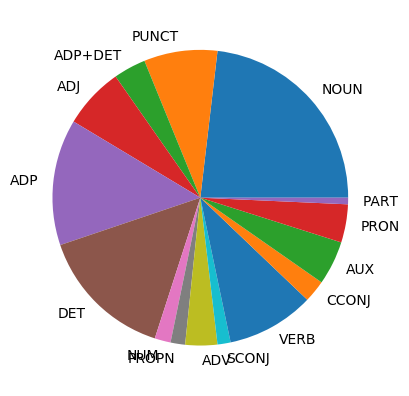
\includegraphics[width=.7\linewidth]{partuttest_img.png}
\caption{distribution des labels}
\end{minipage}
\end{figure} \subparagraph{Données de train \\ }  
 Nombre de phrases : 803\\ 
\begin{figure}[H] \begin{minipage}{0.48\textwidth} \centering \begin{tabular}{|l || *{11 }{|c} |} \hline
Mot & Apparitions  \\ \hline
\begin{verb} de \end{verb} &1114\\ \hline
\begin{verb} , \end{verb} &1016\\ \hline
\begin{verb} . \end{verb} &750\\ \hline
\begin{verb} la \end{verb} &683\\ \hline
\begin{verb} et \end{verb} &544\\ \hline
\begin{verb} l' \end{verb} &486\\ \hline
\begin{verb} des \end{verb} &432\\ \hline
\begin{verb} à \end{verb} &404\\ \hline
\begin{verb} d' \end{verb} &397\\ \hline
\begin{verb} le \end{verb} &385\\ \hline

\end{tabular}
\caption{ Mots les plus utilisés dans le set partut(train) } \label{Fig:muw}\end{minipage} 
\begin{minipage}{0.48\textwidth} \centering
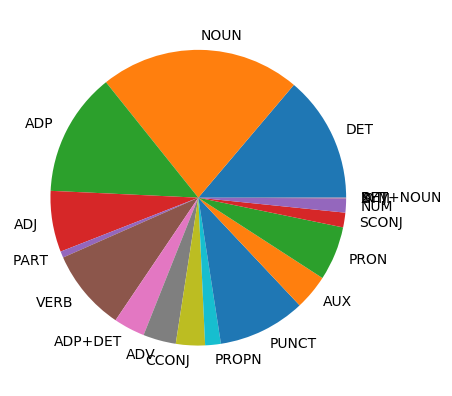
\includegraphics[width=.7\linewidth]{partuttrain_img.png}
\caption{distribution des labels}
\end{minipage}
\end{figure}


\clearpage \subsection{gsd } 
 \begin{itemize} 
 \item[Présentation :] Phrases variées

 \item[Pourcentage de mots hors vocabulaire : ]1.359
 \item[KL-Divergence :]0.409
 \end{itemize}  \subparagraph{Données de test \\ }  
 Nombre de phrases : 416\\ 
\begin{figure}[H] \begin{minipage}{0.48\textwidth} \centering \begin{tabular}{|l || *{11 }{|c} |} \hline
Mot & Apparitions  \\ \hline
\begin{verb} , \end{verb} &489\\ \hline
\begin{verb} de \end{verb} &426\\ \hline
\begin{verb} . \end{verb} &353\\ \hline
\begin{verb} la \end{verb} &222\\ \hline
\begin{verb} et \end{verb} &182\\ \hline
\begin{verb} l' \end{verb} &171\\ \hline
\begin{verb} à \end{verb} &168\\ \hline
\begin{verb} __DIGIT__ \end{verb} &166\\ \hline
\begin{verb} le \end{verb} &155\\ \hline
\begin{verb} les \end{verb} &127\\ \hline

\end{tabular}
\caption{ Mots les plus utilisés dans le set gsd(test) } \label{Fig:muw}\end{minipage} 
\begin{minipage}{0.48\textwidth} \centering
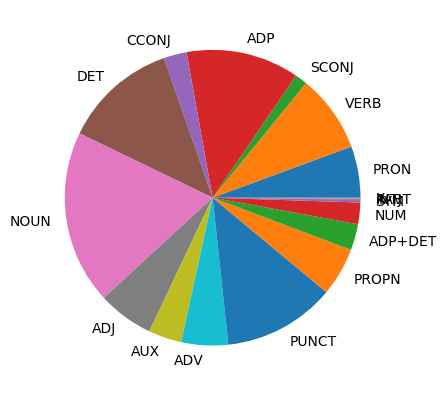
\includegraphics[width=.7\linewidth]{gsdtest_img.png}
\caption{distribution des labels}
\end{minipage}
\end{figure} \subparagraph{Données de train \\ }  
 Nombre de phrases : 14450\\ 
\begin{figure}[H] \begin{minipage}{0.48\textwidth} \centering \begin{tabular}{|l || *{11 }{|c} |} \hline
Mot & Apparitions  \\ \hline
\begin{verb} de \end{verb} &16964\\ \hline
\begin{verb} , \end{verb} &16595\\ \hline
\begin{verb} . \end{verb} &13359\\ \hline
\begin{verb} la \end{verb} &8676\\ \hline
\begin{verb} et \end{verb} &7148\\ \hline
\begin{verb} __DIGIT__ \end{verb} &7095\\ \hline
\begin{verb} le \end{verb} &6389\\ \hline
\begin{verb} à \end{verb} &6216\\ \hline
\begin{verb} l' \end{verb} &5864\\ \hline
\begin{verb} en \end{verb} &4793\\ \hline

\end{tabular}
\caption{ Mots les plus utilisés dans le set gsd(train) } \label{Fig:muw}\end{minipage} 
\begin{minipage}{0.48\textwidth} \centering
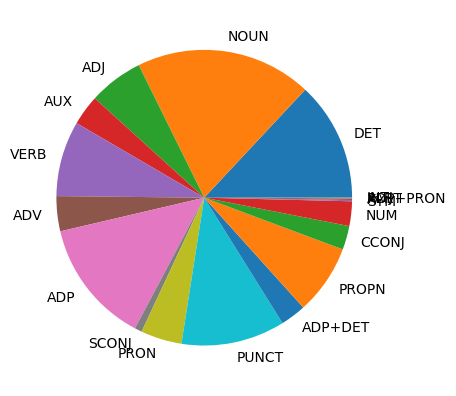
\includegraphics[width=.7\linewidth]{gsdtrain_img.png}
\caption{distribution des labels}
\end{minipage}
\end{figure}

\clearpage
\subsection{foot } 
 \begin{itemize} 
 \item[Présentation :] Ensemble de tweets parlant de football

 \end{itemize}  \subparagraph{Données de test \\ }  
 Nombre de phrases : 743\\ 
\begin{figure}[H] \begin{minipage}{0.48\textwidth} \centering \begin{tabular}{|l || *{11 }{|c} |} \hline
Mot & Apparitions  \\ \hline
\begin{verb} __MENTION__ \end{verb} &549\\ \hline
\begin{verb} la \end{verb} &433\\ \hline
\begin{verb} __SHARP__ \end{verb} &395\\ \hline
\begin{verb} Juventus \end{verb} &368\\ \hline
\begin{verb} : \end{verb} &338\\ \hline
\begin{verb} de \end{verb} &325\\ \hline
\begin{verb} ! \end{verb} &314\\ \hline
\begin{verb} le \end{verb} &257\\ \hline
\begin{verb} , \end{verb} &247\\ \hline
\begin{verb} __URL__ \end{verb} &226\\ \hline

\end{tabular}
\caption{ Mots les plus utilisés dans le set foot(test) } \label{Fig:muw}\end{minipage} 
\begin{minipage}{0.48\textwidth} \centering
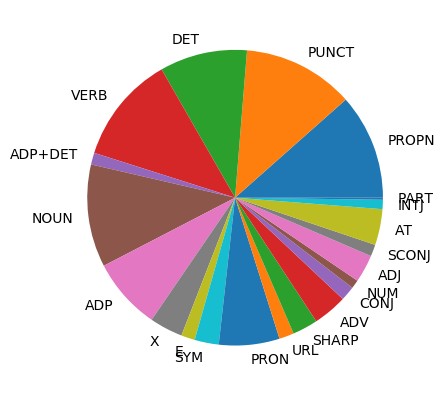
\includegraphics[width=.7\linewidth]{foottest_img.png}
\caption{distribution des labels}
\end{minipage}
\end{figure}


 \subsection{natdis } 
 \begin{itemize} 
 \item[Présentation :] Ensemble de tweets

 \end{itemize}  \subparagraph{Données de test \\ }  
 Nombre de phrases : 622\\ 
\begin{figure}[H] \begin{minipage}{0.48\textwidth} \centering \begin{tabular}{|l || *{11 }{|c} |} \hline
Mot & Apparitions  \\ \hline
\begin{verb} de \end{verb} &994\\ \hline
\begin{verb} __URL__ \end{verb} &469\\ \hline
\begin{verb} __DIGIT__ \end{verb} &411\\ \hline
\begin{verb} terre \end{verb} &338\\ \hline
\begin{verb} __SHARP__ \end{verb} &300\\ \hline
\begin{verb} tremblement \end{verb} &295\\ \hline
\begin{verb} : \end{verb} &285\\ \hline
\begin{verb} chaleur \end{verb} &244\\ \hline
\begin{verb} au \end{verb} &220\\ \hline
\begin{verb} vague \end{verb} &206\\ \hline

\end{tabular}
\caption{ Mots les plus utilisés dans le set natdis(test) } \label{Fig:muw}\end{minipage} 
\begin{minipage}{0.48\textwidth} \centering
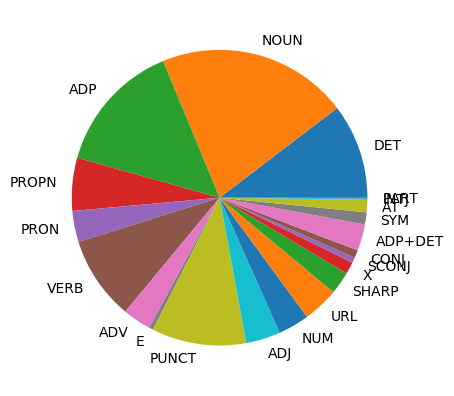
\includegraphics[width=.7\linewidth]{natdistest_img.png}
\caption{distribution des labels}
\end{minipage}
\end{figure}

\onehalfspacing

\section{Présentation du code}
Le code est regroupé dans les fichiers suivants:
\begin{description}
\item[helpers.py] Regroupe des fonctions utiles pour le chargement des
  données ou le test des résultats.
\item[tex\_data\_describe.py et tex\_result\_describe.py] Regroupe des fonctions
  utile pour (respectivement) décrire les données ou les
  résultats vers un ou plusieurs fichiers \LaTeX
\item[modele.py] fournit une interface commune aux différents
  classifieurs. 
\item[multiclass\_perceptron.py] Le perceptron multiclasse du TP5.
\item[modele\_tp5.py] Le perceptron utilisé avec les features du TP
  5.
\item[modele\_pj\_distrib.py] Inclut le modèle de perceptron
  implémenteant les 
  features proposées dans le sujet du projet, incluant les
  \emph{distributional features}.
\item[modele\_pj\_nodistrib.py] Même chose que modele\_pj\_distrib,
  sans les \emph{distributional features}
\item[modeles\_sklearn.py] Utilise deux implémentations de
  classifieurs provenant de la bibliothèque SKLearn.
\end{description}

\subsection{Description des classifieurs}
Les classifieurs possèdent tous la même interface, qui est indiquée
dans {\verb modele.py } \\ 
L'algorithme de classification utilisé pour tous les modèles (hors
ceux  provenant du
module {\verb modeles_sklearn } ) est le perceptron implémenté
dans {\verb multiclass_perceptron } Ainsi, seules les features sont
différentes. \\ Chaque feature est décrite en fonction de la
phrase $sentence$ , et du mot $w$ dont il faut prédire le label, qui
est situé à la position $pos$ dans la phrase. 
% TODO : mettre paragraph

\paragraph{} {\verb Modele_tp5 } 

Ce modèle implémente les features proposées lors du tp 5, qui sont les
suivantes : \\

\begin{itemize}
\item Le mot $w$
\item Les trois derniers caractères de $w$
\item Le premier caractère de $w$
\item Le dernier caractère de $w$
\item un booléen indiquant si le premier caractère est une lettre
  majuscule 
\item un booléen indiquant si tout le mot est écrit en majuscule
\item Le mot précédent dans la phrase
\item Le mot situé à $pos - 2$ dans la phrase.
\item Le mot suivant dans la phrase
\item Le mot situé à $pos + 2$ dans la phrase.
\end{itemize}

Ces features sont implémentées dans la fonction
{\verb build_sparse2 }, et le fichier contenant le Modele est
{\verb modele_tp5.py }.


\paragraph{} {\verb Modele_projet } et {\verb Modele_nodistrib } \\
Implémentent les features proposées dans le sujet du projet : 
\begin{itemize}
\item $w$ 
\item Les deux mots précédant est suivant $w$
\item Le nombre de mots avant $w$ dans la phrase
\item Le nombre de mots suivant $w$ dans la phrase
\item Un booléen indiquant si le mot se finit par un s
\item Un ensemble de booléens, indiquants respectivement si :
  \begin{itemize}
  \item le mot contient un chiffre
  \item le mot contient un tiret
  \item le mot est écrit en majuscules
  \item le mot se finit en {\verb -é }
  \item le mot se finit en {\verb -er }
  \item le mot se finit en {\verb -ant }
  \end{itemize}
\item les \emph{ distributional features }. Elles sont est composées de deux
  features, qu'on appellera respectivement ``distribution à
  droite'' et ``distribution à gauche''.\\
  Pour chaque mot $w$, on regarde le mot juste à droite $c$ (resp.juste à
  gauche), et on calcule le nombre de fois où le nombre de couples
  $w c$ (resp $c w$) apparaît dans le corpus de test. \\
  Les deux features sont égales à ce nombre. On se limite à calculer
  le nombre d'apparitions de ces couples pour $c$ faisant partie des
  10 mots les plus utilisés.
\end{itemize}
La classe {\verb Modele_nodistrib } n'implémente pas les \emph{
  distributional features}. \\
Les deux classes se trouvent respectivement dans
{\verb modele_pj_distrib } et {\verb modele_ph_nodistrib }

\paragraph{} {\verb Modele_sklearn_Perceptron } et {\verb Modele_SKLearn_SVM }
\\
Les features sont construites à partir des informations suivantes :
\begin{itemize}
\item $w$
\item un booléen indiquant si $w$ est écrit en lettres majuscules
\item un booléen indiquant si $w$ commence par une lettre majuscule
\item les trois dernières lettres du mot
\item les deux dernières lettres du mot
\item les trois premières lettres du mot
\item Le mot précédent
\item Le mot suivant
\item un booléen indiquant si le mot est un nombre
\item un booléen indiquant si le mot contient des lettres majuscules  
\end{itemize}

Le dictionnaire représentant les features est donné à une instance de
la classe {\verb DictVectorizer }, qui ``transformera'' ces features
en une forme acceptable pour le classifieur. Ensuite, la
classification sera réalisée par une instance de {\verb Perceptron} ou
  de {\verb LinearSVC }.



  

  

\subsection{Présentation du perceptron}
\section{Résultats}
\begin{figure}[H] \begin{adjustbox}{width=\textwidth} \begin{centering} \begin{tabular}{ | l || *{ 6}{c|c|c||} } \hline 
& \multicolumn{3}{|c|}{ ftb } & \multicolumn{3}{|c|}{ gsd } & \multicolumn{3}{|c|}{ partut } & \multicolumn{3}{|c|}{ pud } & \multicolumn{3}{|c|}{ sequoia } & \multicolumn{3}{|c|}{ spoken }  \\ \hline 
& OOV & AMB & GEN & OOV & AMB & GEN & OOV & AMB & GEN & OOV & AMB & GEN & OOV & AMB & GEN & OOV & AMB & GEN   \\ \hline \hline 
foot  & 22.59 & 80.79 & 62.63
 & 22.22 & 73.40 & 64.74
 & 34.42 & 54.63 & 52.56
 & 34.42 & 54.63 & 52.56
 & 25.72 & 66.45 & 55.48
 & 27.65 & 70.13 & 46.27
 \\ \hline 
ftb  & 72.59 & 91.46 & 92.68
 & 72.65 & 88.20 & 88.76
 & 61.63 & 70.21 & 75.75
 & 61.63 & 70.21 & 75.75
 & 66.23 & 86.56 & 83.22
 & 35.81 & 70.89 & 55.14
 \\ \hline 
gsd  & 66.30 & 86.74 & 87.80
 & 79.51 & 89.87 & 91.60
 & 59.11 & 73.77 & 75.92
 & 59.11 & 73.77 & 75.92
 & 64.67 & 84.70 & 81.58
 & 36.56 & 74.00 & 56.92
 \\ \hline 
natdis  & 24.25 & 87.42 & 76.99
 & 39.30 & 85.03 & 76.20
 & 41.62 & 71.63 & 62.23
 & 41.62 & 71.63 & 62.23
 & 38.50 & 81.83 & 67.66
 & 22.28 & 75.64 & 48.98
 \\ \hline 
partut  & 71.15 & 87.56 & 88.66
 & 64.13 & 89.98 & 88.42
 & 62.11 & 73.64 & 79.56
 & 62.11 & 73.64 & 79.56
 & 68.76 & 86.0 & 81.39
 & 41.48 & 74.19 & 61.07
 \\ \hline 
pud  & 58.28 & 81.36 & 83.36
 & 69.32 & 81.76 & 85.86
 & 59.18 & 65.35 & 71.88
 & 59.18 & 65.35 & 71.88
 & 63.58 & 77.23 & 77.47
 & 40.57 & 75.02 & 58.29
 \\ \hline 
sequoia  & 68.74 & 89.43 & 89.53
 & 72.59 & 90.56 & 90.70
 & 61.19 & 75.90 & 76.44
 & 61.19 & 75.90 & 76.44
 & 67.85 & 88.33 & 86.57
 & 38.93 & 73.47 & 57.38
 \\ \hline 
spoken  & 45.03 & 70.93 & 75.45
 & 45.68 & 72.81 & 77.75
 & 50.0 & 61.08 & 65.96
 & 50.0 & 61.08 & 65.96
 & 48.07 & 64.16 & 65.23
 & 65.22 & 81.94 & 81.24
 \\ \hline 
 \end{tabular} \end{centering} \end{adjustbox} \caption{ taux de réussite} \end{figure} 
\begin{figure}[H] \begin{adjustbox}{width=\textwidth} \begin{centering} \begin{tabular}{ | l || *{ 6}{c|c|c||} } \hline 
& \multicolumn{3}{|c|}{ ftb } & \multicolumn{3}{|c|}{ gsd } & \multicolumn{3}{|c|}{ partut } & \multicolumn{3}{|c|}{ pud } & \multicolumn{3}{|c|}{ sequoia } & \multicolumn{3}{|c|}{ spoken }  \\ \hline 
& OOV & AMB & GEN & OOV & AMB & GEN & OOV & AMB & GEN & OOV & AMB & GEN & OOV & AMB & GEN & OOV & AMB & GEN   \\ \hline \hline 
foot  & 13.47 & 80.21 & 58.29
 & 13.71 & 74.31 & 58.93
 & 14.60 & 67.05 & 38.91
 & 14.60 & 67.05 & 38.91
 & 18.35 & 69.62 & 50.86
 & 12.84 & 70.73 & 36.64
 \\ \hline 
ftb  & 57.25 & 90.61 & 90.62
 & 54.09 & 88.13 & 85.70
 & 45.02 & 79.49 & 70.04
 & 45.02 & 79.49 & 70.04
 & 57.30 & 88.14 & 80.99
 & 26.35 & 71.93 & 49.89
 \\ \hline 
gsd  & 44.92 & 86.04 & 83.73
 & 53.99 & 90.25 & 88.23
 & 40.80 & 81.26 & 69.16
 & 40.80 & 81.26 & 69.16
 & 49.33 & 87.75 & 77.87
 & 24.71 & 74.97 & 50.72
 \\ \hline 
natdis  & 19.37 & 84.76 & 72.73
 & 32.50 & 84.97 & 73.67
 & 21.33 & 76.79 & 49.79
 & 21.33 & 76.79 & 49.79
 & 37.48 & 83.17 & 65.19
 & 15.51 & 73.34 & 41.80
 \\ \hline 
partut  & 57.69 & 84.72 & 86.44
 & 38.04 & 87.76 & 84.01
 & 49.48 & 85.0 & 75.70
 & 49.48 & 85.0 & 75.70
 & 54.57 & 88.11 & 79.52
 & 30.65 & 74.57 & 54.87
 \\ \hline 
pud  & 35.91 & 80.44 & 78.99
 & 47.38 & 81.61 & 81.72
 & 38.22 & 74.45 & 64.49
 & 38.22 & 74.45 & 64.49
 & 47.70 & 78.99 & 73.20
 & 27.12 & 76.38 & 51.08
 \\ \hline 
sequoia  & 53.70 & 88.82 & 86.19
 & 53.42 & 91.08 & 86.37
 & 38.68 & 82.37 & 68.17
 & 38.68 & 82.37 & 68.17
 & 53.94 & 89.65 & 83.42
 & 26.41 & 74.98 & 51.14
 \\ \hline 
spoken  & 35.20 & 70.98 & 72.92
 & 30.24 & 73.40 & 75.42
 & 28.31 & 68.34 & 58.92
 & 28.31 & 68.34 & 58.92
 & 41.95 & 69.77 & 66.45
 & 43.29 & 80.79 & 74.94
 \\ \hline 
 \end{tabular} \end{centering} \end{adjustbox} \caption{ Pourcentage de réussite du classifieur courant} \end{figure} 
\begin{figure}[H] \begin{adjustbox}{width=\textwidth} \begin{centering} \begin{tabular}{ | l || *{ 6}{c|c|c||} } \hline 
& \multicolumn{3}{|c|}{ ftb } & \multicolumn{3}{|c|}{ gsd } & \multicolumn{3}{|c|}{ partut } & \multicolumn{3}{|c|}{ pud } & \multicolumn{3}{|c|}{ sequoia } & \multicolumn{3}{|c|}{ spoken }  \\ \hline 
& OOV & AMB & GEN & OOV & AMB & GEN & OOV & AMB & GEN & OOV & AMB & GEN & OOV & AMB & GEN & OOV & AMB & GEN   \\ \hline \hline 
foot  & 14.37 & 80.23 & 57.75
 & 14.95 & 74.20 & 59.46
 & 17.32 & 73.26 & 42.60
 & 17.32 & 73.26 & 42.60
 & 15.44 & 67.25 & 46.71
 & 13.93 & 64.54 & 35.78
 \\ \hline 
ftb  & 57.33 & 90.74 & 90.42
 & 58.03 & 87.98 & 86.25
 & 51.32 & 82.50 & 73.40
 & 51.32 & 82.50 & 73.40
 & 55.33 & 86.96 & 80.09
 & 29.42 & 68.89 & 50.58
 \\ \hline 
gsd  & 46.01 & 86.41 & 83.86
 & 59.20 & 90.37 & 89.37
 & 47.18 & 84.35 & 72.50
 & 47.18 & 84.35 & 72.50
 & 48.63 & 86.23 & 76.65
 & 26.80 & 71.44 & 50.56
 \\ \hline 
natdis  & 19.64 & 84.88 & 72.24
 & 34.46 & 84.62 & 73.20
 & 26.30 & 79.71 & 53.43
 & 26.30 & 79.71 & 53.43
 & 39.06 & 80.80 & 63.80
 & 18.32 & 67.69 & 44.00
 \\ \hline 
partut  & 57.69 & 85.47 & 86.36
 & 40.21 & 89.27 & 84.89
 & 54.26 & 86.89 & 79.68
 & 54.26 & 86.89 & 79.68
 & 58.67 & 88.82 & 80.11
 & 34.81 & 69.25 & 54.51
 \\ \hline 
pud  & 37.90 & 80.49 & 79.07
 & 48.28 & 82.36 & 82.67
 & 45.19 & 76.09 & 68.41
 & 45.19 & 76.09 & 68.41
 & 45.79 & 77.63 & 71.91
 & 29.13 & 72.80 & 51.23
 \\ \hline 
sequoia  & 52.02 & 89.24 & 85.77
 & 55.16 & 90.11 & 86.48
 & 44.59 & 84.92 & 72.22
 & 44.59 & 84.92 & 72.22
 & 52.50 & 89.90 & 83.30
 & 28.47 & 72.02 & 51.12
 \\ \hline 
spoken  & 34.76 & 70.36 & 71.55
 & 29.85 & 73.23 & 75.43
 & 35.80 & 71.35 & 62.23
 & 35.80 & 71.35 & 62.23
 & 41.21 & 66.75 & 63.19
 & 48.28 & 77.75 & 74.22
 \\ \hline 
 \end{tabular} \end{centering} \end{adjustbox} \caption{ taux de réussite} \end{figure} 
\section{Conclusion}
\end{document}
